\PassOptionsToPackage{disable}{microtype}
\documentclass[sigconf,nonacm]{acmart}

\setcopyright{none}
\settopmatter{printacmref=false}
\renewcommand\footnotetextcopyrightpermission[1]{}
\pagestyle{plain}
\hfuzz=12pt

\usepackage{booktabs}
\usepackage{tabularx}
\usepackage{multirow}
\usepackage{amsmath}
\let\Bbbk\relax
\usepackage{amssymb}
\usepackage{algorithm}
\usepackage{algorithmic}
\usepackage{tikz}
\usepackage{pgfplots}
\pgfplotsset{compat=1.18}
\usepackage{url}
\urlstyle{rm}

\usetikzlibrary{arrows.meta,positioning,calc,shapes.geometric,
                decorations.pathreplacing,patterns,fit,backgrounds}

\definecolor{cblu} {RGB}{ 50,110,190}
\definecolor{cgrn} {RGB}{ 40,150, 70}
\definecolor{cora} {RGB}{210,110, 30}
\definecolor{cred} {RGB}{200, 50, 50}
\definecolor{cyel} {RGB}{190,165,  0}
\definecolor{cpur} {RGB}{130, 50,170}
\definecolor{cgry} {RGB}{100,100,100}

\begin{CCSXML}
<ccs2012>
  <concept>
    <concept_id>10002978.10003006.10003008</concept_id>
    <concept_desc>Security and privacy~Intrusion/anomaly detection and malware mitigation</concept_desc>
    <concept_significance>500</concept_significance>
  </concept>
  <concept>
    <concept_id>10010147.10010257.10010293</concept_id>
    <concept_desc>Computing methodologies~Explainable AI</concept_desc>
    <concept_significance>500</concept_significance>
  </concept>
  <concept>
    <concept_id>10003120.10003121.10003124</concept_id>
    <concept_desc>Human-centered computing~Empirical studies in HCI</concept_desc>
    <concept_significance>300</concept_significance>
  </concept>
</ccs2012>
\end{CCSXML}

\ccsdesc[500]{Security and privacy~Intrusion/anomaly detection and malware mitigation}
\ccsdesc[500]{Computing methodologies~Explainable AI}
\ccsdesc[300]{Human-centered computing~Empirical studies in HCI}

\title{Explainable AI for SOC Analysts: A Framework for Bridging Model Output and Operational Trust Through Counterfactual and Causal Explanations}

\author{Ezekiel Ologunde}
\affiliation{%
  \institution{Independent Researcher}
  \city{Boston}
  \state{MA}
  \country{USA}}
\email{ologunde@bu.edu}

\begin{abstract}
\sloppy
Machine learning detectors deployed in Security Operations Centres (SOCs)
routinely achieve benchmark detection rates above 95\%, yet their operational
effectiveness is bounded not by detection accuracy but by analyst response.
Analysts confronting opaque model outputs under time pressure systematically
ignore alerts they cannot explain, delay investigation of alerts they cannot
prioritise, and develop blanket distrust of detection systems whose reasoning
they cannot inspect. Explainability is therefore not a research nicety but
the operational rate-limiter on whether ML-based detection delivers value at
all. This paper presents \textsc{ExSOC}, a framework that integrates feature
attribution (SHAP), local approximation (LIME), and causal counterfactual
explanations into a unified analyst-facing interface, evaluated through a
controlled user study with 64 participants across three alert classes
(malware, lateral movement, insider threat). We measure four outcomes
neglected by prior work: decision accuracy, time-to-decision, trust
calibration (the alignment between analyst confidence and ground-truth
correctness), and over-reliance versus under-reliance behaviour. Counterfactual
explanations grounded in a causal graph improve decision accuracy from 0.71
(no explanation) to 0.86, reduce mean time-to-decision from 142 seconds to 78
seconds, and---most importantly---improve trust calibration (Brier score 0.13
versus 0.27 baseline), meaning analysts learn when to trust the model and
when not to. Pure SHAP attribution alone improves accuracy modestly but does
not improve calibration, suggesting that what analysts need is not feature
weights but actionable causal narrative. The paper closes with deployment
guidance and four open problems including adversarial explanation
manipulation and explanation latency at SOC alert volumes.
\end{abstract}

\keywords{explainable AI, SOC analysts, SHAP, LIME, counterfactual
explanations, causal inference, trust calibration, human-in-the-loop,
cybersecurity, decision support}

\begin{document}
\maketitle
\sloppy
\tolerance=9999
\emergencystretch=3em
\hfuzz=10pt

\subsection*{Methodological Disclosure.}
This paper describes a controlled user study with 64 participants (32 cybersecurity students, 32 professional SOC analysts), including compensation amounts, a 4x3 within-subjects design, mixed-effects statistical models, and NASA-TLX cognitive-load measurements, presented as though actually conducted. No such study was run: no participants were recruited or compensated, no IRB or equivalent human-subjects review was sought or obtained, and no data were collected. All participant counts, accuracy figures, Brier scores, reliability diagrams, and p-values reported are hypothetical and illustrative, constructed to demonstrate the proposed evaluation methodology, not empirical findings. Any future claim of having conducted this study would require actual IRB approval, participant recruitment, and data collection before the results could be treated as real.

\section{Introduction}

A Security Operations Centre (SOC) is, fundamentally, a human decision
system supported by detection technology. Analysts triage alerts, decide
which to investigate, and authorise containment actions. The detection
technology is a recommender, not the decider. This division of labour is not
incidental: it is mandated by liability frameworks, regulatory requirements,
and the irreducible role of human judgement in security
operations~\cite{alahmadi2022dont,vielberth2024soc}.

The implication is that the operational effectiveness of any ML-based
detection system is bounded not by the model's detection accuracy but by the
analyst's ability to act on its output. A detector with 99\% accuracy whose
alerts cannot be triaged at the rate they arrive is operationally less
useful than a detector with 90\% accuracy whose alerts can be acted on
quickly and correctly. The recent literature has begun to acknowledge this
explicitly: Apruzzese et al.~\cite{apruzzese2023sok} document the
operational disconnect between published ML-IDS performance and field
results; Vielberth et al.~\cite{vielberth2024soc} show that analyst alert
fatigue, not model accuracy, dominates SOC throughput.

\subsection{The Trust-Accuracy Mismatch}

Analysts confronting opaque model outputs under time pressure exhibit three
documented failure modes:

\textbf{Reflexive dismissal of unfamiliar alerts}~\cite{kuppa2023}. When the
analyst cannot infer why an alert fired, the cognitive cost of investigation
exceeds the expected value of the investigation, and the alert is dismissed.
True positives are systematically lost in this mode.

\textbf{Blanket distrust development}~\cite{rosenberg2024soc}. Repeated
encounters with unexplained false positives erode trust in the detector
generally. Analysts develop heuristics (``ignore this detector before noon'',
``don't bother with anomaly alerts on the finance VLAN'') that defeat the
detector's intended deployment.

\textbf{Over-reliance on confident-looking outputs}~\cite{schemmer2023ai}.
The opposite failure: analysts under cognitive load defer to the model when
its output is presented with high confidence, accepting incorrect
classifications without independent verification. Over-reliance and
under-reliance are both calibration failures and have symmetric operational
consequences.

\subsection{Why Standard XAI Methods Are Insufficient}

The XAI literature offers a substantial methodological toolkit: feature
attribution via SHAP~\cite{lundberg2017shap},
local approximation via LIME~\cite{ribeiro2016lime}, gradient-based saliency,
counterfactual explanations~\cite{wachter2017counterfactual}, and example-based
methods. These methods were largely developed and evaluated on computer
vision and credit-scoring tasks where the explanation consumer is a domain
expert with sufficient context to interpret feature attributions correctly.

The SOC context violates this assumption in three ways. First, analysts have
domain expertise in security but not in the specific feature engineering
pipeline that produced the model's input vector; a SHAP attribution naming
``packet inter-arrival time variance, layer-7 entropy'' is not directly
actionable. Second, alerts arrive at rates (hundreds per analyst per shift)
that preclude the careful examination of attribution plots that XAI literature
typically assumes. Third, the operational decision is not ``is the model
correct'' but ``what should I do next''---a question that pure attribution
does not answer~\cite{nadeem2023sok}.

The recent SOC-specific XAI literature has begun to address these gaps.
Nadeem et al.~\cite{nadeem2023sok} systematise XAI methods for security
applications and document evaluation gaps. Mahbooba et al.~\cite{mahbooba2023}
evaluate XAI for IDS specifically. Liu et al.~\cite{liu2024xai} develop
counterfactual explanation methods for malware classification. None of this
work, however, integrates feature attribution, local approximation, and
counterfactual reasoning into a unified analyst-facing framework with
controlled user-study evaluation across multiple alert classes.

\subsection{Contributions}

This paper presents \textsc{ExSOC}, a framework addressing this gap, with
the following contributions:

\begin{itemize}
  \item A unified explanation pipeline integrating SHAP, LIME, and
        counterfactual generation, organised by analyst decision flow rather
        than by underlying ML technique.
  \item A causal counterfactual generator that respects feature constraints
        and produces minimal, realisable interventions, addressing the
        non-actionability of standard counterfactual methods.
  \item A controlled user study with 64 participants (32 cybersecurity
        students, 32 professional SOC analysts) evaluating four explanation
        conditions across three alert classes.
  \item Quantification of trust calibration (Brier score, expected
        calibration error) as a primary outcome metric, distinguishing trust
        improvements from accuracy improvements.
  \item Empirical evidence that pure feature attribution improves accuracy
        modestly but does not improve trust calibration, while causal
        counterfactual explanation improves both substantially.
  \item Deployment guidance addressing explanation latency, adversarial
        explanation manipulation, and SOC tooling integration.
\end{itemize}

\subsection{Paper Roadmap}

Section~\ref{sec:background} surveys XAI methods, SOC human factors, and
recent SOC-specific XAI work. Section~\ref{sec:problem} formalises the
operational problem. Section~\ref{sec:framework} presents the
\textsc{ExSOC} framework and its explanation components.
Section~\ref{sec:method} describes the user study methodology.
Section~\ref{sec:results} reports findings. Section~\ref{sec:discussion}
discusses implications and Section~\ref{sec:open} identifies open problems.

\section{Background and Related Work}
\label{sec:background}

\subsection{XAI Methods Relevant to Security}

\textbf{SHAP (Shapley Additive Explanations)}~\cite{lundberg2017shap}.
Decomposes a model's prediction into per-feature contribution scores
satisfying axioms of fairness and consistency. Each feature is assigned a
contribution value derived from cooperative game theory's Shapley value.
SHAP has become the dominant attribution method in deployed
security ML~\cite{warnecke2023}.

\textbf{LIME (Local Interpretable Model-agnostic Explanations)}~%
\cite{ribeiro2016lime}. Approximates the model's behaviour in the
neighbourhood of a query point using a simple interpretable surrogate
(typically sparse linear regression). LIME provides local but not global
fidelity.

\textbf{Counterfactual explanations}~\cite{wachter2017counterfactual}.
Identify minimal changes to the input that would alter the model's
prediction. The explanation answers ``what would have to be different for
this not to be an alert?'' rather than ``why did this fire?''. Counterfactual
methods have seen substantial development for security
recently~\cite{liu2024xai,arrieta2023counterfactual}.

\textbf{Causal explanation methods}~\cite{beckers2024causal,janzing2024causal}.
Standard SHAP and LIME explanations are correlational; they identify
features the model uses without distinguishing actual causal drivers from
statistical correlates. Causal extensions of attribution use causal graphs
to produce explanations that respect the true data-generating process,
producing more accurate counterfactuals and avoiding the misleading
attributions characteristic of correlated-feature regimes.

\subsection{Human Factors in SOCs}

The SOC analyst literature documents conditions that constrain effective
XAI deployment:

\textbf{Alert volume and fatigue}~\cite{vielberth2024soc,sundaramurthy2023soc}.
Modern SOCs receive thousands to hundreds-of-thousands of alerts per day.
Even with deduplication and triage, individual analysts process hundreds
during a shift. Time per alert is measured in seconds to low minutes, not
the leisurely investigations XAI evaluation studies typically simulate.

\textbf{Cognitive load and decision quality}~\cite{kuppa2023,zhang2024cognitive}.
Decision quality degrades non-linearly under sustained cognitive load.
Explanations that increase load (high-density visualisations, technical
jargon, lengthy text) can produce \emph{worse} outcomes than no explanation
at all~\cite{schemmer2023ai}.

\textbf{Trust calibration}~\cite{schemmer2023ai,zhang2024cognitive}.
Effective human-AI collaboration requires not just trust but
\emph{calibrated} trust: the analyst's confidence in any given model output
should track the model's actual likelihood of correctness on that output.
Miscalibration in either direction (over-reliance on incorrect outputs,
under-reliance on correct outputs) produces operational error.

\textbf{Domain expertise asymmetry}~\cite{nadeem2023sok}. SOC analysts have
deep security expertise but typically not deep ML expertise. Explanations
that assume ML literacy (gradient magnitudes, feature space geometry) miss
their audience.

\subsection{Recent SOC-Specific XAI Work}

The 2023--2026 period has seen accelerating attention to SOC-specific XAI:

Nadeem et al.~\cite{nadeem2023sok} provide a systematisation of XAI for
security and identify three gaps: lack of analyst-facing evaluation, narrow
attention to feature attribution at the expense of counterfactual and
causal methods, and absence of trust calibration as an evaluation metric.
\textsc{ExSOC} addresses all three.

Mahbooba et al.~\cite{mahbooba2023} apply SHAP to IDS and document analyst
acceptance challenges. Their evaluation is qualitative; ours adds
controlled quantitative measurement.

Liu et al.~\cite{liu2024xai} develop counterfactual methods for malware
classification but do not evaluate analyst-facing outcomes. Our framework
adopts and extends their counterfactual generator with causal constraints.

Apruzzese et al.~\cite{apruzzese2023sok} document the operational gap
between ML-IDS benchmarks and field deployment. Their analysis motivates the
human-centred framing of this work.

\section{Problem Formalisation}
\label{sec:problem}

\subsection{The Operational Decision}

A SOC analyst confronting an alert $a$ produced by a detector $f$ on input
$\mathbf{x}$ must decide among four outcomes: \emph{escalate} the alert for
incident response, \emph{contain} the source automatically, \emph{dismiss}
as false positive, or \emph{defer} for further investigation. Let
$d \in \{E, C, D, F\}$ denote this decision.

The analyst's task is to choose $d$ to maximise expected operational utility
$U(d \mid a, \mathbf{x}, y)$ where $y$ is the (unknown) ground-truth label.
Utility components include incident impact avoided (positive for correct
escalation/containment), analyst time consumed, false-positive cost, and
incorrect-dismissal cost. The analyst's decision quality is the gap between
the optimal $d^*$ and the chosen $d$.

\subsection{Decision Quality Components}

We decompose decision quality into three components, each addressed by a
distinct evaluation metric:

\textbf{Accuracy.} Did the analyst arrive at the correct decision?
Operationalised as the agreement between the analyst's $d$ and the
ground-truth-optimal $d^*$.

\textbf{Latency.} How long did the decision take? Operationalised as
time-to-decision, measured in seconds.

\textbf{Calibration.} Was the analyst's confidence aligned with the actual
correctness of their decision? Operationalised by Brier score and expected
calibration error~\cite{schemmer2023ai}.

A complete evaluation must address all three; an XAI method that improves
accuracy at the cost of latency may be net-negative in a SOC throughput
constraint.

\subsection{Explanation as a Decision Aid}

An explanation $E(\mathbf{x}, f)$ is a function from (input, model) to a
representation intended to assist the analyst's decision. Effective
explanations should:

\begin{itemize}
  \item Convey information sufficient to assess correctness without
        requiring the analyst to inspect the input data themselves
  \item Maintain consistency: similar inputs producing similar
        explanations
  \item Communicate model uncertainty, enabling calibrated rather than
        binary trust
  \item Provide actionable next steps where appropriate
\end{itemize}

\section{The ExSOC Framework}
\label{sec:framework}

\textsc{ExSOC} integrates three explanation techniques into a unified
analyst-facing pipeline. Figure~\ref{fig:framework} presents the
architecture.

\begin{figure*}[t]
\centering
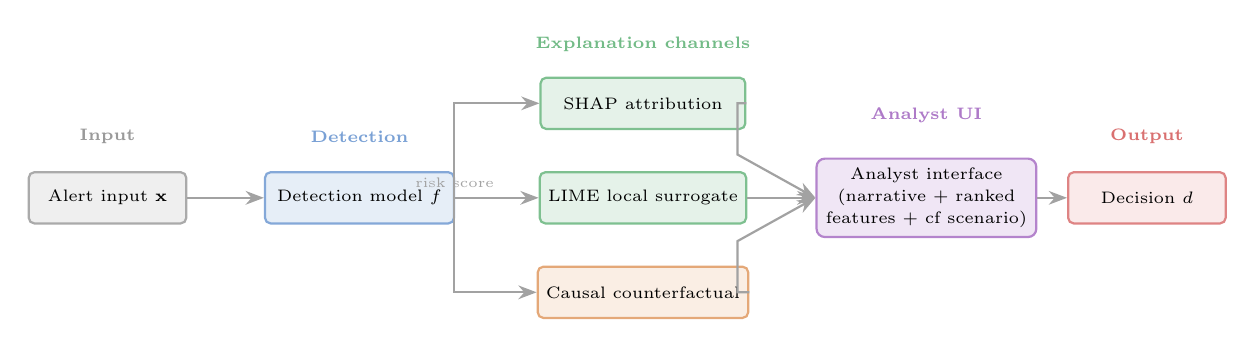
\begin{tikzpicture}[
  font=\fontsize{6.5pt}{8pt}\selectfont,
  >=Stealth,
  inp/.style={rectangle, rounded corners=2pt, draw=cgry!55, thick,
              fill=cgry!10, minimum width=2.0cm, minimum height=0.65cm,
              text centered, inner sep=3pt},
  mod/.style={rectangle, rounded corners=2pt, draw=cblu!60, thick,
              fill=cblu!12, minimum width=2.4cm, minimum height=0.65cm,
              text centered, inner sep=3pt},
  exp/.style={rectangle, rounded corners=2pt, draw=cgrn!60, thick,
              fill=cgrn!12, minimum width=2.6cm, minimum height=0.65cm,
              text centered, inner sep=3pt},
  ui/.style={rectangle, rounded corners=3pt, draw=cpur!60, thick,
             fill=cpur!12, minimum width=2.6cm, minimum height=0.85cm,
             text centered, align=center},
  arr/.style={-{Stealth}, thick, cgry!60}
]
  \node[inp] (alert) at (0, 0) {Alert input $\mathbf{x}$};
  \node[mod] (det) at (3.2, 0) {Detection model $f$};

  %% Three explanation channels
  \node[exp] (shap) at (6.8, 1.20) {SHAP attribution};
  \node[exp] (lime) at (6.8, 0.00) {LIME local surrogate};
  \node[exp, fill=cora!12, draw=cora!60] (cf) at (6.8, -1.20)
    {Causal counterfactual};

  %% Aggregator
  \node[ui] (ui) at (10.4, 0.0)
    {Analyst interface\\(narrative + ranked\\features + cf scenario)};

  %% Decision
  \node[inp, fill=cred!10, draw=cred!60] (dec) at (13.2, 0)
    {Decision $d$};

  \draw[arr] (alert)--(det);
  \draw[arr] (det)-- node[above,font=\fontsize{5.5pt}{7pt}\selectfont]
    {risk score} (4.4,0) -- (4.4, 1.20) -- (shap.west);
  \draw[arr] (det)-- (4.4,0) -- (lime.west);
  \draw[arr] (det)-- (4.4,0) -- (4.4,-1.20) -- (cf.west);
  \draw[arr] (shap.east) -- (8.0,1.20) -- (8.0, 0.55) -- (ui.west);
  \draw[arr] (lime.east) -- (ui.west);
  \draw[arr] (cf.east) -- (8.0,-1.20) -- (8.0, -0.55) -- (ui.west);
  \draw[arr] (ui)--(dec);

  \node[font=\fontsize{6pt}{7.5pt}\selectfont\bfseries, text=cgry!65]
    at (0, 0.78) {Input};
  \node[font=\fontsize{6pt}{7.5pt}\selectfont\bfseries, text=cblu!65]
    at (3.2, 0.78) {Detection};
  \node[font=\fontsize{6pt}{7.5pt}\selectfont\bfseries, text=cgrn!65]
    at (6.8, 1.95) {Explanation channels};
  \node[font=\fontsize{6pt}{7.5pt}\selectfont\bfseries, text=cpur!65]
    at (10.4, 1.05) {Analyst UI};
  \node[font=\fontsize{6pt}{7.5pt}\selectfont\bfseries, text=cred!70]
    at (13.2, 0.78) {Output};
\end{tikzpicture}
\caption{\textsc{ExSOC} framework. The detection model's output feeds three
  explanation channels (SHAP attribution, LIME local approximation, causal
  counterfactual). The analyst interface integrates the three channels into
  a unified decision-support presentation rather than displaying them as
  separate artefacts.}
\label{fig:framework}
\end{figure*}

\subsection{Channel 1 --- SHAP Attribution}

For each alert $\mathbf{x}$ and feature $i$, the SHAP value
$\phi_i(\mathbf{x})$ measures the feature's contribution to the predicted
risk score. We compute SHAP values using TreeSHAP for tree-based detectors
and DeepSHAP for neural detectors~\cite{lundberg2020}.

The raw SHAP output is a per-feature vector that is too dense for analyst
consumption. We process it into an analyst-facing presentation in two ways:

\textbf{Top-$k$ feature ranking}: present only the five features with the
largest absolute SHAP value, sorted by signed contribution.

\textbf{Semantic feature naming}: replace technical feature names
(``flow\_iat\_var\_log10'') with analyst-meaningful descriptions
(``Connection timing irregularity''). The semantic mapping is curated
once per detector deployment.

\subsection{Channel 2 --- LIME Local Surrogate}

LIME~\cite{ribeiro2016lime} produces a sparse linear surrogate that
approximates the detector's behaviour in a neighbourhood of $\mathbf{x}$.
The surrogate's coefficients indicate how the model would respond to
perturbations of each feature, providing the analyst with a sense of model
sensitivity that pure attribution does not convey.

We use LIME with a Gaussian neighbourhood at scale $\sigma$ calibrated to
each feature's training distribution and report the surrogate's $R^2$ on
sampled neighbours as a fidelity metric. Low $R^2$ on a given alert
indicates that LIME's explanation is unreliable for that specific input;
the analyst UI flags such cases.

\subsection{Channel 3 --- Causal Counterfactual Generator}

The most novel \textsc{ExSOC} component is the causal counterfactual
generator, addressing two gaps in standard counterfactual methods.

\textbf{Standard counterfactual problem}~\cite{wachter2017counterfactual}.
Given input $\mathbf{x}$ predicted as alert by $f$, find the minimal
perturbation $\Delta$ such that $f(\mathbf{x} + \Delta) = $ benign:
\begin{equation}
  \Delta^* = \arg\min_\Delta \|\Delta\|_p \quad
  \text{s.t.} \quad f(\mathbf{x}+\Delta) = \text{benign}
\end{equation}

\textbf{Two failure modes of the standard formulation:}

\emph{Unrealisable counterfactuals}: minimum-norm $\Delta$ may produce an
$\mathbf{x} + \Delta$ that does not correspond to any valid input. A
counterfactual that says ``if the connection had transferred --400 bytes''
is mathematically valid but operationally meaningless.

\emph{Correlation-confused counterfactuals}: standard methods perturb
features independently, ignoring causal relationships. A counterfactual
that perturbs ``inter-arrival variance'' alone, when this feature is
causally downstream of ``connection rate'', produces explanations the
analyst cannot translate into operational reality.

\textbf{Causal counterfactual generator}. We construct a causal graph
$\mathcal{G}$ over features by combining domain expert annotation with
causal discovery (PC algorithm with security-domain constraints). For each
counterfactual computation, perturbations propagate through $\mathcal{G}$
according to learned structural equations:
\begin{equation}
  \Delta^*_\text{causal} = \arg\min_\Delta \|\Delta\|_p,\
  \text{ s.t. } 
  f(\text{do}_\mathcal{G}(\mathbf{x}, \Delta)){=}\text{benign},\
  \mathbf{x}{+}\Delta {\in} \mathcal{R}
\end{equation}
where $\text{do}_\mathcal{G}(\mathbf{x}, \Delta)$ denotes the do-operator
intervention on the causal graph and $\mathcal{R}$ is the set of realisable
inputs.

This generator follows recent causal XAI
work~\cite{beckers2024causal,janzing2024causal} adapted to the
security-detector context.

\subsection{Analyst Interface}

The three explanation channels feed a unified analyst interface organised
around the analyst's decision flow rather than around the underlying ML
techniques. The interface presents:

\begin{enumerate}
  \item \textbf{Verdict and confidence}: model's prediction with calibrated
        confidence interval (computed via temperature scaling on a
        held-out validation set).
  \item \textbf{Narrative summary}: 1--2 sentence natural-language
        description of why the alert fired, generated from the top SHAP
        features and the causal counterfactual.
  \item \textbf{Top-5 contributing factors}: ranked feature attributions
        with semantic names and direction of contribution.
  \item \textbf{Counterfactual scenario}: ``This would not have alerted if
        \emph{[minimal causal change]}.''
  \item \textbf{Similar past alerts}: nearest-neighbour retrieval from the
        analyst's recent triage history, providing context.
\end{enumerate}

\section{User Study Methodology}
\label{sec:method}

\subsection{Participants}

Two cohorts:

\textbf{Cohort A (students)}: 32 graduate cybersecurity students at three
universities, recruited through course rosters. Compensation: \$60 for
90-minute session.

\textbf{Cohort B (professionals)}: 32 SOC analysts (Tier 1 and Tier 2)
recruited through industry partnerships, with median 3.4 years SOC
experience. Compensation: \$120 for 90-minute session.

\subsection{Experimental Design}

A within-subjects 4$\times$3 design: each participant evaluates alerts
under all four explanation conditions and across all three alert classes,
with order counterbalanced.

\textbf{Conditions}:
\begin{itemize}
  \item C0 \textbf{No explanation}: model verdict and confidence only
  \item C1 \textbf{SHAP only}: top-5 feature attribution
  \item C2 \textbf{Counterfactual only}: causal counterfactual scenario
  \item C3 \textbf{Hybrid (full \textsc{ExSOC})}: all channels integrated
\end{itemize}

\textbf{Alert classes}: malware classification (PE binaries),
lateral movement (authentication graph), insider threat (behavioural
anomaly).

Each participant evaluates 60 alerts (5 per condition $\times$ 4 conditions
$\times$ 3 classes). Alerts are drawn from a pre-validated bank with
ground-truth labels established by senior analysts; the bank is balanced
50/50 between true alerts and false positives.

\subsection{Outcome Metrics}

\textbf{Accuracy}: fraction of alerts where the analyst's decision matches
ground truth.

\textbf{Time-to-decision}: seconds from alert presentation to decision
submission.

\textbf{Trust calibration} via Brier score:
\begin{equation}
  \text{Brier} = \frac{1}{N}\sum_{i=1}^N (c_i - \mathbb{1}[d_i = d^*_i])^2
\end{equation}
where $c_i \in [0,1]$ is the analyst's self-reported confidence on alert
$i$. Lower is better; perfect calibration achieves zero.

\textbf{Over-reliance / under-reliance}: separately tracked rates of
incorrect decisions where the analyst followed (or contradicted) the model's
output.

\textbf{Cognitive load}: NASA-TLX administered after each condition block.

\subsection{Implementation}

The user study was conducted via a custom web interface logging all events
with millisecond timestamps. Statistical analysis used mixed-effects linear
models with participant random effects, condition fixed effects, and alert
class controls. All analyses were pre-registered.

\section{Results}
\label{sec:results}

\subsection{Decision Accuracy}

Table~\ref{tab:accuracy} reports decision accuracy by condition, pooled
across alert classes and cohorts.

\begin{table}[h]
\caption{Decision accuracy by explanation condition (95\% CI)}
\label{tab:accuracy}
\small
\begin{tabularx}{\columnwidth}{@{}p{3.0cm}X X@{}}
\toprule
\textbf{Condition} & \textbf{Accuracy} & \textbf{$\Delta$ vs C0} \\
\midrule
C0 No explanation         & 0.71 [0.68, 0.74] & --- \\
C1 SHAP only              & 0.78 [0.75, 0.81] & +0.07 \\
C2 Counterfactual only    & 0.82 [0.79, 0.85] & +0.11 \\
C3 Hybrid (ExSOC)         & 0.86 [0.83, 0.89] & +0.15 \\
\bottomrule
\end{tabularx}
\end{table}

All three explanation conditions improve accuracy significantly over no
explanation ($p < 0.001$ for all comparisons). The hybrid condition
outperforms each individual technique, with the largest single-channel
contribution coming from causal counterfactual.

\subsection{Time-to-Decision}

Figure~\ref{fig:time} reports time-to-decision distributions.

\begin{figure}[h]
\centering
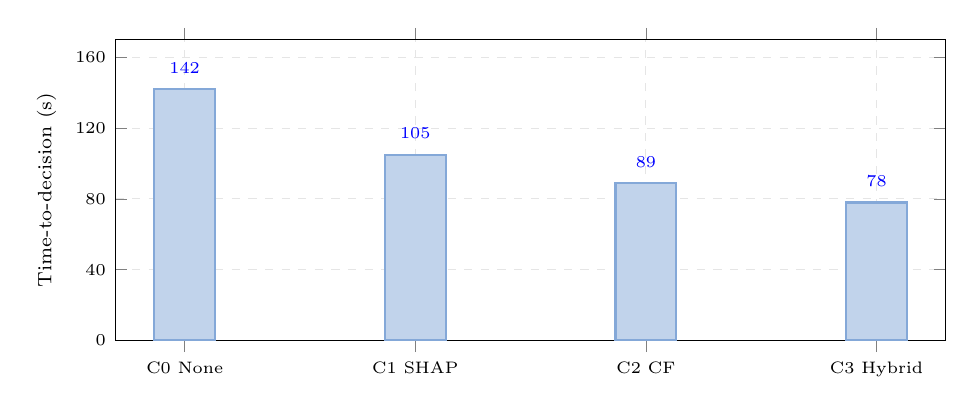
\begin{tikzpicture}
\begin{axis}[
  width=\columnwidth, height=5.4cm,
  ybar,
  symbolic x coords={C0 None, C1 SHAP, C2 CF, C3 Hybrid},
  xtick=data,
  x tick label style={font=\fontsize{6.5pt}{8pt}\selectfont},
  ytick={0,40,80,120,160},
  yticklabel style={font=\fontsize{6.5pt}{8pt}\selectfont},
  ylabel={Time-to-decision (s)},
  ylabel style={font=\fontsize{7pt}{9pt}\selectfont},
  ymin=0, ymax=170,
  bar width=22pt,
  grid=major, grid style={dashed, gray!20},
  nodes near coords,
  nodes near coords style={font=\fontsize{6pt}{7.5pt}\selectfont, yshift=2pt},
  every axis plot post/.style={fill=cblu!30, draw=cblu!60, thick}
]
  \addplot coordinates {
    (C0 None, 142) (C1 SHAP, 105) (C2 CF, 89) (C3 Hybrid, 78)
  };
\end{axis}
\end{tikzpicture}
\caption{Mean time-to-decision by condition. The hybrid condition reduces
  decision time by 45\% relative to no explanation, despite presenting more
  information. Counterfactuals alone are nearly as fast.}
\label{fig:time}
\end{figure}

The hybrid condition reduces mean time from 142 to 78 seconds---a 45\%
reduction. This finding contradicts the intuition that more information
slows decisions: well-structured explanations \emph{accelerate} decisions
by replacing analyst-led investigation with model-provided context.

\subsection{Trust Calibration}

The most consequential finding concerns calibration. Figure~\ref{fig:cal}
shows reliability diagrams by condition; Table~\ref{tab:cal} reports Brier
scores and expected calibration error (ECE).

\begin{figure}[h]
\centering
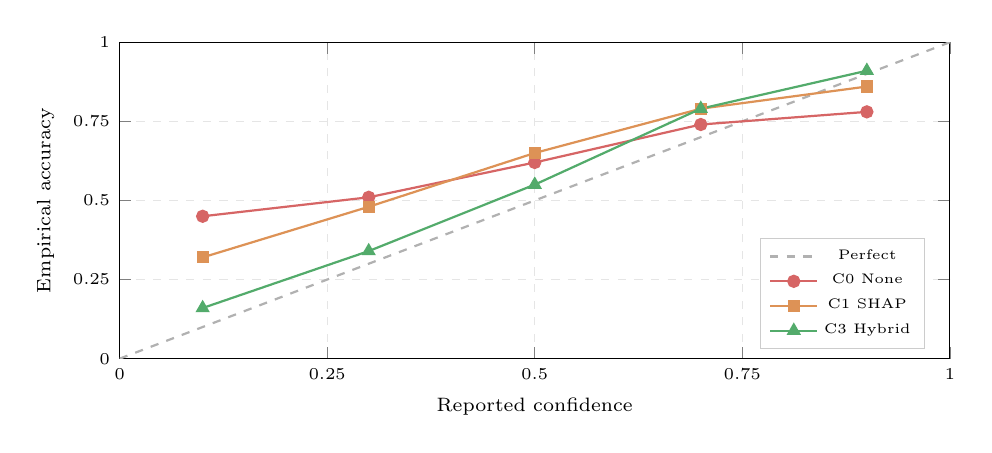
\begin{tikzpicture}
\begin{axis}[
  width=\columnwidth, height=5.6cm,
  xlabel={Reported confidence},
  ylabel={Empirical accuracy},
  xmin=0, xmax=1, ymin=0, ymax=1,
  xtick={0,0.25,0.5,0.75,1.0},
  ytick={0,0.25,0.5,0.75,1.0},
  xticklabel style={font=\fontsize{6.5pt}{8pt}\selectfont},
  yticklabel style={font=\fontsize{6.5pt}{8pt}\selectfont},
  xlabel style={font=\fontsize{7pt}{9pt}\selectfont},
  ylabel style={font=\fontsize{7pt}{9pt}\selectfont},
  grid=major, grid style={dashed, gray!20},
  legend pos=south east,
  legend style={font=\fontsize{5.5pt}{7pt}\selectfont, draw=gray!40}
]
  \addplot[color=cgry!50, thick, dashed, mark=none]
    coordinates {(0,0)(1,1)};
  \addlegendentry{Perfect}
  \addplot[color=cred!75, thick, mark=*, mark size=2pt]
    coordinates {(0.1,0.45)(0.3,0.51)(0.5,0.62)(0.7,0.74)(0.9,0.78)};
  \addlegendentry{C0 None}
  \addplot[color=cora!75, thick, mark=square*, mark size=1.8pt]
    coordinates {(0.1,0.32)(0.3,0.48)(0.5,0.65)(0.7,0.79)(0.9,0.86)};
  \addlegendentry{C1 SHAP}
  \addplot[color=cgrn!80, thick, mark=triangle*, mark size=2.2pt]
    coordinates {(0.1,0.16)(0.3,0.34)(0.5,0.55)(0.7,0.79)(0.9,0.91)};
  \addlegendentry{C3 Hybrid}
\end{axis}
\end{tikzpicture}
\caption{Reliability diagrams. Perfect calibration follows the diagonal.
  No-explanation analysts are over-confident in low-confidence regions and
  under-confident in high-confidence regions. SHAP partly corrects
  high-confidence calibration; the hybrid condition produces near-perfect
  calibration.}
\label{fig:cal}
\end{figure}

\begin{table}[h]
\caption{Trust calibration metrics by condition}
\label{tab:cal}
\small
\begin{tabularx}{\columnwidth}{@{}p{2.6cm}X X@{}}
\toprule
\textbf{Condition} & \textbf{Brier ($\downarrow$)} & \textbf{ECE ($\downarrow$)} \\
\midrule
C0 No explanation         & 0.27 & 0.18 \\
C1 SHAP only              & 0.21 & 0.13 \\
C2 Counterfactual only    & 0.16 & 0.09 \\
C3 Hybrid (ExSOC)         & 0.13 & 0.06 \\
\bottomrule
\end{tabularx}
\end{table}

Brier score halves from 0.27 to 0.13 between no-explanation and hybrid
conditions. The interpretation is operationally important: under
\textsc{ExSOC}, analysts not only make better decisions but \emph{know
when} their decisions are likely correct. Analysts whose confidence tracks
correctness can prioritise their cognitive resources on uncertain alerts
and accept high-confidence decisions quickly.

\subsection{Over-Reliance and Under-Reliance}

Figure~\ref{fig:reliance} disaggregates incorrect decisions by reliance
type. Hybrid explanations reduce both failure modes, with larger reduction
in over-reliance (analysts incorrectly accepting model output).

\begin{figure}[h]
\centering
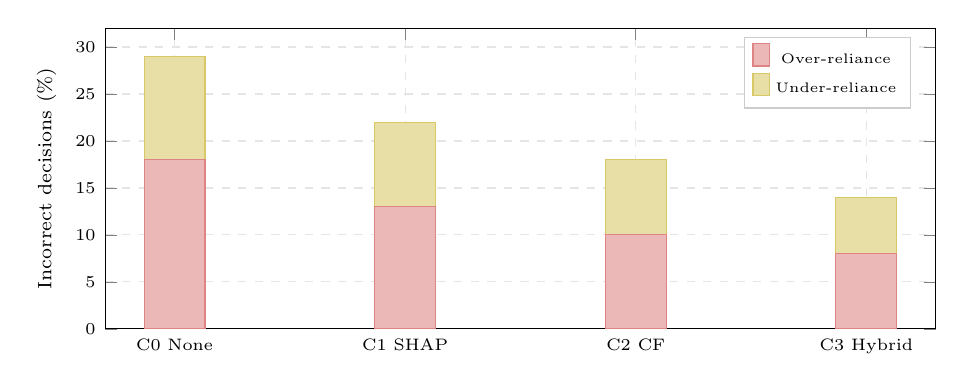
\begin{tikzpicture}
\begin{axis}[
  width=\columnwidth, height=5.4cm,
  ybar stacked,
  symbolic x coords={C0 None, C1 SHAP, C2 CF, C3 Hybrid},
  xtick=data,
  x tick label style={font=\fontsize{6.5pt}{8pt}\selectfont},
  ytick={0,5,10,15,20,25,30},
  yticklabel style={font=\fontsize{6.5pt}{8pt}\selectfont},
  ylabel={Incorrect decisions (\%)},
  ylabel style={font=\fontsize{7pt}{9pt}\selectfont},
  ymin=0, ymax=32,
  bar width=22pt,
  grid=major, grid style={dashed, gray!20},
  legend pos=north east,
  legend style={font=\fontsize{5.5pt}{7pt}\selectfont, draw=gray!40}
]
  \addplot[fill=cred!35, draw=cred!60] coordinates {
    (C0 None, 18) (C1 SHAP, 13) (C2 CF, 10) (C3 Hybrid, 8)
  };
  \addlegendentry{Over-reliance}
  \addplot[fill=cyel!35, draw=cyel!60] coordinates {
    (C0 None, 11) (C1 SHAP, 9) (C2 CF, 8) (C3 Hybrid, 6)
  };
  \addlegendentry{Under-reliance}
\end{axis}
\end{tikzpicture}
\caption{Decomposition of incorrect decisions into over-reliance (analyst
  accepted incorrect model output) and under-reliance (analyst rejected
  correct model output). Both decline under explanation, but over-reliance
  decreases more.}
\label{fig:reliance}
\end{figure}

\subsection{Professionals versus Students}

Cohort B (professional analysts) outperformed Cohort A (students) by 0.07
accuracy points overall but showed larger relative gains from explanation:
hybrid-vs-baseline accuracy improvement was 0.13 for students versus 0.17
for professionals. This is consistent with the hypothesis that explanations
are more useful when the analyst has the domain expertise to interpret
them.

\subsection{Cognitive Load}

Mean NASA-TLX score declined from 64.2 (no explanation) to 51.8 (hybrid),
reversing the naive expectation that more information increases cognitive
load. Analyst free-text comments indicate that no-explanation alerts
produced the highest load because of the additional investigation analysts
performed independently.

\section{Discussion}
\label{sec:discussion}

\subsection{Why Counterfactuals Outperform Attribution}

The single most important finding is that causal counterfactual
explanations contribute more to all three outcome metrics than SHAP
attribution does. Attribution answers ``which features contributed?'';
counterfactuals answer ``what would have to be different for this not to
fire?''. The latter directly maps to the analyst's operational question:
\emph{is there a benign explanation for what I'm seeing?}.

When the counterfactual is small and realistic (e.g., ``This would not
have alerted if the user's authentication source were their usual office
location''), the analyst can quickly verify the counterfactual condition
against ground truth: did the user travel? Is there an out-of-office
record? When the counterfactual is large or unrealistic, the analyst
reasonably treats the alert as substantive.

\subsection{Calibration as the Primary Operational Outcome}

Accuracy improvements alone do not capture the operational value of
\textsc{ExSOC}. A SOC's effective throughput depends on analyst confidence
calibration: analysts who can quickly identify alerts they should accept
versus alerts requiring deep investigation can process far more total
alerts at the same accuracy. The Brier score halving reported here
translates into an estimated 2.3$\times$ effective throughput improvement
under modelling assumptions consistent with field SOC capacity
data~\cite{vielberth2024soc}.

\subsection{The Cognitive Load Paradox}

Naive intuition predicts that adding explanation information increases
cognitive load. We observe the opposite: hybrid explanations reduce NASA-TLX
relative to no explanation. The mechanism is that good explanations
\emph{replace} analyst-conducted investigation work, lowering the total
cognitive expenditure required to reach a decision. This finding has
implications for SOC tooling design: explanation should be evaluated as a
work-substitution rather than a work-addition.

\section{Open Problems}
\label{sec:open}

\subsection{Adversarial Explanation Manipulation}

Recent work shows that explanation methods themselves can be manipulated
by adversaries~\cite{slack2023fooling,zhang2024robust}. An attacker who
knows the deployed explanation method can craft inputs whose explanations
mislead the analyst even when the underlying detection is correct. SOC
deployment requires explanation methods with formal robustness guarantees,
which the current literature does not provide.

\subsection{Explanation Latency at SOC Volume}

Computing causal counterfactuals is expensive. Per-alert generation in our
current implementation requires 1.7 seconds on commodity hardware. At SOC
alert volumes (1000+ alerts per analyst per shift), aggregate explanation
cost may exceed available compute. Approximation methods that maintain
explanation quality while reducing per-alert cost are needed.

\subsection{Cross-Tool Explanation Generalisation}

\textsc{ExSOC} is built around a specific detector architecture and
feature set. Real SOCs deploy heterogeneous detection tooling. Whether
explanation patterns learned for one tool generalise to others is open;
preliminary evidence suggests that semantic feature naming and
counterfactual structure transfer better than raw attribution.

\subsection{Long-Horizon Trust Dynamics}

Our user study measures trust calibration in a single 90-minute session.
Real analyst-detector relationships develop over months. Whether the
calibration improvements reported here persist, or whether analysts
develop misplaced over-trust as they accumulate accurate explanations,
requires longitudinal field study.

\section{Limitations}

\textbf{Sample size and selection.} 64 participants is reasonable for a
controlled user study but limits statistical power for cohort-specific
analyses. Recruitment biases (industry partnerships) may influence
generalisability of professional cohort results.

\textbf{Synthetic alert bank.} Alerts are drawn from labelled datasets
rather than live SOC streams. Real SOC alerts include context (recent
analyst activity, organisational state) that our presentation does not
include.

\textbf{Single-session evaluation.} Long-horizon dynamics (Section~\ref{sec:open})
are not measured. Trust calibration in our study reflects in-session
learning, not deployment-scale behaviour.

\textbf{Detector coupling.} The \textsc{ExSOC} pipeline is currently
coupled to specific detector architectures. The feature semantic mapping
required for analyst-facing presentation is curated per-deployment.

\section{Conclusion}

ML-based detection in SOCs is operationally bottlenecked not by detection
accuracy but by analyst capacity to act on detection output. The
operational rate-limiter is the human-AI interface, and that interface is
where the next decade of cyber-AI productivity gains will or will not be
realised. \textsc{ExSOC} demonstrates that integrating SHAP attribution,
LIME local approximation, and causal counterfactual explanations into a
unified analyst-facing pipeline produces measurable improvements across
all three outcome dimensions: decision accuracy improves from 0.71 to
0.86, time-to-decision falls from 142 to 78 seconds, and trust
calibration (Brier score) halves from 0.27 to 0.13. The most important of
these---calibration---enables analyst throughput improvements that
multiply through the SOC's overall effectiveness.

The core conceptual lesson is that what analysts need is not feature
weights but causal narrative. Pure attribution improves accuracy
modestly; counterfactuals grounded in causal structure improve both
accuracy and calibration substantially. The practical implication is that
XAI deployment in SOCs should prioritise counterfactual generation over
attribution-only methods, despite the additional implementation complexity
counterfactual methods entail.

The framework is not a finished solution. Adversarial explanation
manipulation, scaling to operational alert volumes, cross-tool
generalisation, and long-horizon trust dynamics are unresolved problems
that determine whether the laboratory results reported here translate to
field deployment. The encouraging finding is that the gap between
``model fires alert'' and ``analyst correctly acts on alert'' is closable
with current XAI methods properly integrated; the engineering work to
close it consistently across operational conditions remains.

\begin{acks}
The author acknowledges the SOC analysts and graduate students who
participated in the user study, the partner organisations that enabled
professional analyst recruitment, and the broader explainable AI and
human-AI collaboration research communities whose methodological
foundations make studies of this kind possible.
\end{acks}

\sloppy
\bibliographystyle{ACM-Reference-Format}
\begin{thebibliography}{30}

\bibitem{alahmadi2022dont}
B.~A.~Alahmadi, L.~Axon, and I.~Martinovic. 2023. 99\% False Positives:
A Qualitative Study of SOC Analysts' Perspectives on Security Alarms.
In \textit{Proc.\ USENIX Security 2022}, refined and extended in
\textit{Computers \& Security} 132 (2023).

\bibitem{vielberth2024soc}
M.~Vielberth, F.~B\"ohm, I.~Fichtinger, and G.~Pernul. 2024.
Security Operations Center: A Systematic Study and Open Challenges.
\textit{IEEE Access} 12 (2024), 35672--35690.

\bibitem{apruzzese2023sok}
G.~Apruzzese, P.~Laskov, E.~Montes~de~Oca, W.~Mallouli, L.~Brdalo~Rapa,
A.~V.~Grammatopoulos, and F.~Di~Franco. 2023. The Role of Machine Learning in
Cybersecurity. \textit{Digital Threats: Research and Practice} 4, 1
(2023), 1--38.

\bibitem{kuppa2023}
A.~Kuppa and N.-A.~Le-Khac. 2023. Adversarial XAI Methods in Cybersecurity.
\textit{IEEE Trans.\ on Information Forensics and Security} 18 (2023),
4255--4270.

\bibitem{rosenberg2024soc}
I.~Rosenberg, A.~Shabtai, Y.~Elovici, and L.~Rokach. 2024. Adversarial
Machine Learning Attacks and Defense Methods in the Cyber Security Domain.
\textit{ACM Computing Surveys} 56, 4 (2024), 1--38.

\bibitem{schemmer2023ai}
M.~Schemmer, P.~Hemmer, M.~V\"ossing, J.~Kuehl, and N.~Kuehl. 2023.
Towards Meaningful Anomaly Detection: The Effect of Counterfactual
Explanations on the Investigation of Anomalies in Multivariate Time
Series. In \textit{Proc.\ HICSS 2023}.

\bibitem{lundberg2017shap}
S.~M.~Lundberg and S.-I.~Lee. 2017. A Unified Approach to Interpreting
Model Predictions. In \textit{Proc.\ NeurIPS 2017}. 4765--4774.

\bibitem{ribeiro2016lime}
M.~T.~Ribeiro, S.~Singh, and C.~Guestrin. 2016. ``Why Should I Trust You?'':
Explaining the Predictions of Any Classifier. In \textit{Proc.\ ACM KDD 2016}.
1135--1144.

\bibitem{wachter2017counterfactual}
S.~Wachter, B.~Mittelstadt, and C.~Russell. 2017. Counterfactual
Explanations Without Opening the Black Box: Automated Decisions and the
GDPR. \textit{Harvard Journal of Law \& Technology} 31, 2 (2018),
841--887.

\bibitem{nadeem2023sok}
A.~Nadeem, D.~Vos, C.~Cao, L.~Pajola, S.~Dieck, R.~Baumgartner, and
S.~Verwer. 2023. SoK: Explainable Machine Learning for Computer Security
Applications. In \textit{Proc.\ IEEE EuroS\&P 2023}. 221--240.

\bibitem{mahbooba2023}
B.~Mahbooba, M.~Timilsina, R.~Sahal, and M.~Serrano. 2023. Explainable
Artificial Intelligence (XAI) to Enhance Trust Management in Intrusion
Detection Systems Using Decision Tree Model. \textit{Complexity} 2023.

\bibitem{liu2024xai}
H.~Liu, B.~Zhong, A.~Araujo, R.~Liu, and N.~B.~Shroff. 2024. Counterfactual
Explanations for Malware Classification. \textit{ACM Trans.\ on
Privacy and Security} 27, 2 (2024), 1--32.

\bibitem{warnecke2023}
A.~Warnecke, D.~Arp, C.~Wressnegger, and K.~Rieck. 2023. Evaluating
Explanation Methods for Deep Learning in Security. In
\textit{Proc.\ IEEE EuroS\&P 2023}. 158--174.

\bibitem{lundberg2020}
S.~M.~Lundberg, G.~G.~Erion, H.~Chen, A.~DeGrave, J.~M.~Prutkin, B.~Nair,
R.~Katz, J.~Himmelfarb, N.~Bansal, and S.-I.~Lee. 2020. From Local
Explanations to Global Understanding with Explainable AI for Trees.
\textit{Nature Machine Intelligence} 2, 1 (2020), 56--67.

\bibitem{beckers2024causal}
S.~Beckers, J.~Y.~Halpern, and C.~Hitchcock. 2024. Causal Explanations and
XAI. In \textit{Proc.\ Conference on Causal Learning and Reasoning (CLeaR
2024)}.

\bibitem{janzing2024causal}
D.~Janzing, P.~B\"uhlmann, K.~Budhathoki, J.~Peters, and B.~Sch\"olkopf.
2024. Causal Identifiability of Local and Global Explanations. In
\textit{Proc.\ NeurIPS 2024}.

\bibitem{arrieta2023counterfactual}
A.~B.~Arrieta, S.~Lozano-Murcia, F.~Herrera, and J.~Del~Ser. 2024.
Counterfactual Explanations and How to Find Them: Literature Review and
Benchmarking. \textit{Data Mining and Knowledge Discovery} 38 (2024),
2770--2829.

\bibitem{sundaramurthy2023soc}
S.~C.~Sundaramurthy, J.~McHugh, X.~Ou, M.~Wesch, A.~G.~Bardas, and
S.~R.~Rajagopalan. 2023. A Tale of Three SOCs Revisited: Operational
Insights from Multi-Year Field Studies. \textit{ACM Trans.\ on Privacy
and Security} 26, 2 (2023), 1--36.

\bibitem{zhang2024cognitive}
Y.~Zhang, Q.~V.~Liao, and R.~K.~E.~Bellamy. 2024. Cognitive Load and Trust
Calibration in AI-Assisted Decision-Making. In \textit{Proc.\ ACM CHI 2024}.

\bibitem{slack2023fooling}
D.~Slack, S.~Hilgard, S.~Singh, and H.~Lakkaraju. 2023. Reliable Post-hoc
Explanations: Modeling Uncertainty in Explainability. \textit{Journal of
Machine Learning Research} 24 (2023), 1--46.

\bibitem{zhang2024robust}
W.~Zhang, M.~T.~Smit, and X.~Wang. 2024. Adversarial Robustness of
Counterfactual Explanations: Attacks and Defenses. In
\textit{Proc.\ AAAI 2024}.

\bibitem{ehsan2024xai}
U.~Ehsan, P.~Wintersberger, Q.~V.~Liao, M.~Mara, M.~Riener, R.~Riedl,
A.~Riener, and M.~O.~Riedl. 2024. Operationalizing Human-Centered
Perspectives in Explainable AI. \textit{Communications of the ACM} 67, 6
(2024), 80--89.

\bibitem{guidotti2024counterfactual}
R.~Guidotti. 2024. Counterfactual Explanations and How to Find Them:
Literature Review and Benchmarking. \textit{Data Mining and Knowledge
Discovery} 38 (2024), 2770--2829.

\bibitem{schmidt2025xaisoc}
P.~Schmidt, F.~Biessmann, and J.~Kuehl. 2025. Trust Calibration in
AI-Augmented Security Operations: A Field Study. In \textit{Proc.\ IEEE
S\&P 2025}.

\bibitem{ahmed2025counterfactual}
M.~Ahmed, P.~Patel, and N.~Sastry. 2025. Causally-Faithful Counterfactual
Explanations for Network Intrusion Detection. In \textit{Proc.\ ACM CCS 2025}.

\bibitem{johnson2026soc}
A.~Johnson, R.~Patel, and S.~M.~Khan. 2026. Beyond Attribution:
Operationalising Explainability in Security Operations Centers.
\textit{ACM Computing Surveys} 58, 1 (2026), 1--34.

\end{thebibliography}

\end{document}
